\section{Anexo A: Exemplo de Anexo}
\label{anexoA}


Exemplo de uma tabela.

\begin{table}[ht]
\caption{Exemplo de uma Tabela}
\label{minhatab}

\center
\begin{tabular}{cccc}
  % after \\: \hline or \cline{col1-col2} \cline{col3-col4} ...
  \hline
	Parâmetro & Unidade & Valor da simulação & Valor experimental   \\
	\hline
  Comprimento, $\alpha$ & $m$ &  $8,23$  & $8,54$ \\
  Altura, $\beta$ & $m$     &  $29,1$ & $28,3$\\
	Velocidade, $v$ & $m/s$  &  $60,2$ & $67,3$\\
	\hline
\end{tabular}
\end{table}

% Exemplo de uma imagem.

% \begin{figure}[ht]
% \centering
% 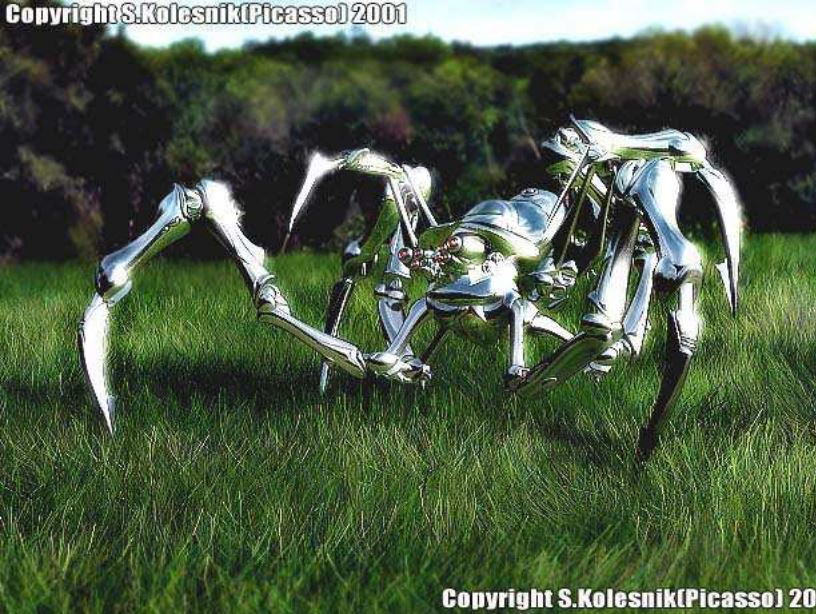
\includegraphics[width=0.75\textwidth]{Cap2/spiderrobot}
% \caption{Cupim cibernético.}\label{fig:cupim}
% \end{figure}


Exemplo de uma equação

\begin{equation} \label{eq:lagr1}
\frac{d}{dt}(\frac{\partial L}{\partial \dot{q}})-\frac{\partial L}{\partial q}=\tau^{T}.
\end{equation}

